
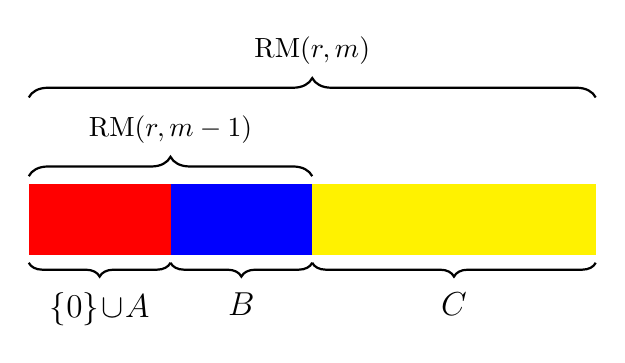
\begin{tikzpicture}[xscale=0.9,yscale=-0.9]

\fill[red] (0,0) rectangle ++(1,1);
\fill[red] (1,0) rectangle ++(1,1);

% \foreach \x in {0,1,...,7} {
%     \fill[gray] (\x+8,0) rectangle ++(1,1);
%   }

\foreach \x in {0,1,...,3} {
    \fill[yellow] (\x+4,0) rectangle ++(1,1);
  }


%\node (c) at (8.5,2) {\large $C$};
%\draw (c1) edge [bend left=5] (c);
%\draw (c2) -- (c);
%\draw (c3) edge [bend right=5] (c);

\foreach \x in {2,3} {
    \fill[blue] (\x,0) rectangle ++(1,1);
}

\draw [
    thick,
    decoration={
        brace,
		%mirror,
		amplitude=7pt,
        raise=0.1cm
    },
    decorate
] (0,0) -- (4,0)
node  [pos=0.5,anchor=north,yshift=1cm] {RM($r,m-1$)}; 

\draw [
    thick,
    decoration={
        brace,
		%mirror,
		amplitude=7pt,
        raise=1.1cm
    },
    decorate
] (0,0) -- (8,0)
node  [pos=0.5,anchor=north,yshift=2cm] {RM($r,m$)};


\draw [
    thick,
    decoration={
        brace,
        mirror,
		amplitude=5pt,
        raise=1cm
    },
    decorate
] (4,0) -- (8,0)
node [pos=0.5,anchor=north,yshift=-1.25cm] {\large $C$}; 

\draw [
    thick,
    decoration={
        brace,
        mirror,
		amplitude=5pt,
        raise=1cm
    },
    decorate
] (2,0) -- (4,0)
node [pos=0.5,anchor=north,yshift=-1.25cm] {\large $B$}; 

\draw [
    thick,
    decoration={
        brace,
		mirror,
		amplitude=5pt,
        raise=1cm
    },
    decorate
] (0,0) -- (2,0)
node [pos=0.5,anchor=north,yshift=-1.25cm] {\large $\{0\} \!\cup\! A$}; 
\end{tikzpicture}